\documentclass[convert={density=300,size=1080x800,outext=.png}]{standalone}

\usepackage{tikz}

\usetikzlibrary{shapes,arrows,positioning,backgrounds,shadows}
% \tikzexternalize

\tikzstyle{decision} = [diamond, draw, fill=white!20, 
    text width=4.5em, text badly centered, node distance=3cm, inner sep=0pt]
\tikzstyle{block} = [rectangle, draw, fill=white!20, 
    text width=8em, text centered, rounded corners, minimum height=2em,node distance=4em]
\tikzstyle{block2} = [rectangle, draw, fill=white!20, 
    text width=8em, text centered, rounded corners, minimum height=2em,node distance=4em,fill=red!20]
\tikzstyle{output} = [rectangle, draw, fill=white!20, 
    text width=8em, text centered, rounded corners, minimum height=2em,node distance=4em,fill=green!20]
% \tikzstyle{easy} = [rectangle, draw, fill=green!40, 
%     text width=5em, text centered, rounded corners, minimum height=4em]
% \tikzstyle{medium} = [rectangle, draw, fill=orange!40, 
%     text width=5em, text centered, rounded corners, minimum height=4em]
% \tikzstyle{hard} = [rectangle, draw, fill=red!40, 
%     text width=5em, text centered, rounded corners, minimum height=4em]
\tikzstyle{line} = [draw, -latex']
\tikzstyle{cloud} = [draw, ellipse,fill=red!20, node distance=3cm,
    minimum height=2em]

\begin{document}
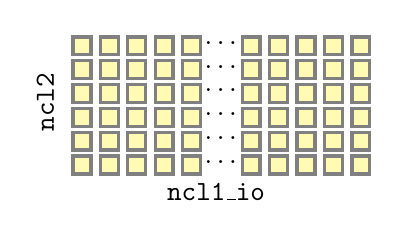
\begin{tikzpicture}
    \node[rotate=90] (ncl1) at (-1em,-4ex) {\texttt{ncl2}};
    \node (ncl2) at (12ex,-11.5ex) {\texttt{ncl1\_io}};

    \foreach \y in {0,1,2,3,4,5}
    {  
            \foreach \x in {0,1,2,3,4}
            {

                \path (\x*2.3ex,\y*-2ex) node (bot_left) {};
                \path (bot_left)+(1.5ex,1.5ex) node (top_right) {};
                \path[draw=black!50,very thick,fill=yellow!30] (bot_left) rectangle (top_right);
            };
            \node (dot) at (12.4ex,\y*-2ex+1ex) {$\ldots$};
            \foreach \x in {0,1,2,3,4}
            {

                \path (14.2ex+\x*2.3ex,\y*-2ex) node (bot_left) {};
                \path (bot_left)+(1.5ex,1.5ex) node (top_right) {};
                \path[draw=black!50,very thick,fill=yellow!30] (bot_left) rectangle (top_right);
            };
    };
    
\end{tikzpicture}
\end{document}